
\documentclass[a4paper,12pt]{article}

\usepackage[margin=1.5cm]{geometry}
\usepackage[T1]{fontenc}
\usepackage{lmodern}
\usepackage{tikz}
\usetikzlibrary{arrows.meta,calc}

\pagestyle{empty}

\begin{document}

\begin{center}
    {\Large\bfseries UML Class Diagram}\\[4pt]
    {\large Leave Inheritance Hierarchy}
\end{center}

\vspace{0.5cm}

\begin{center}
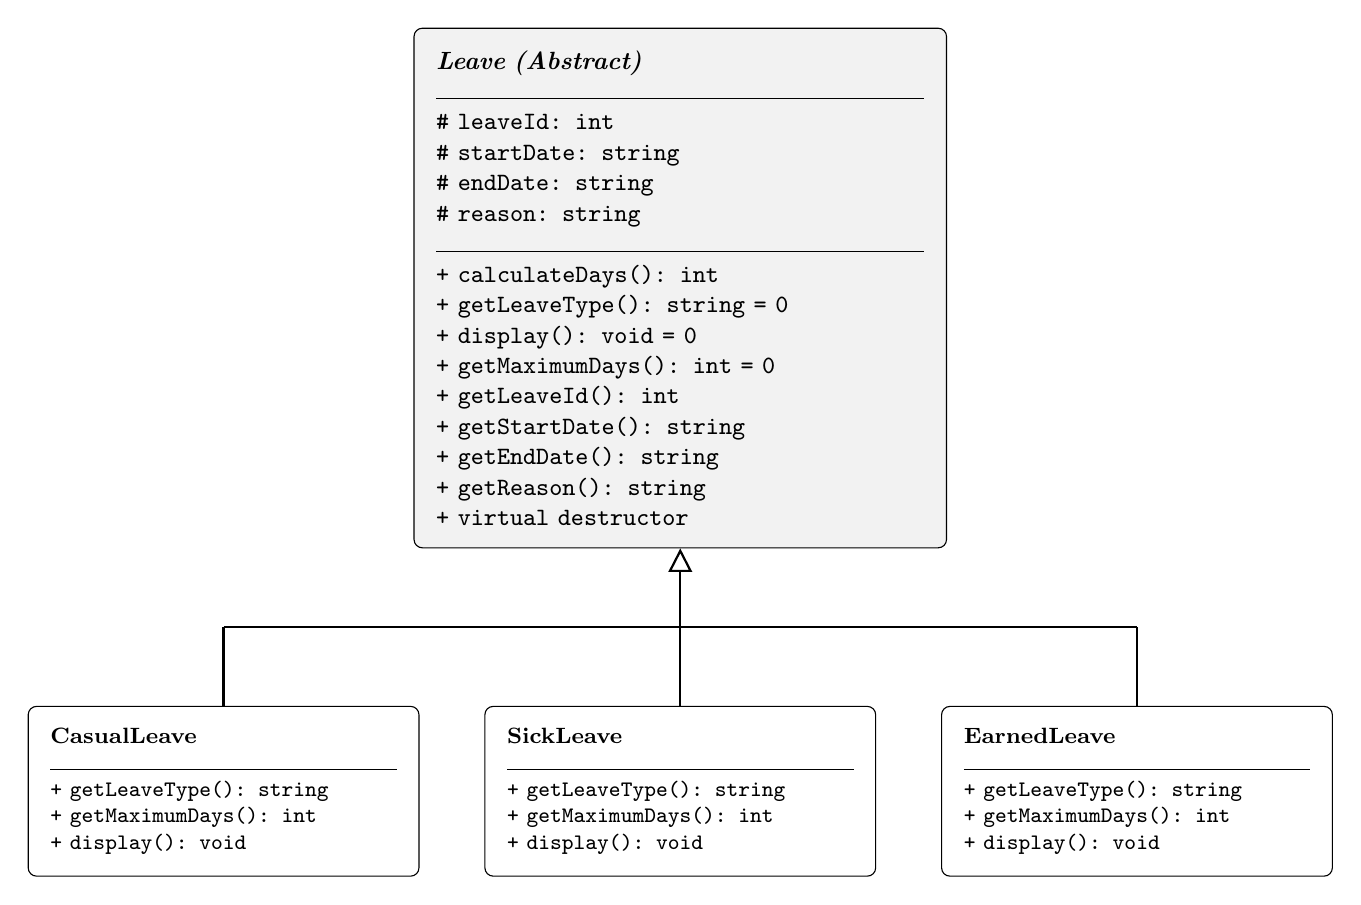
\begin{tikzpicture}[
    classbox/.style={
        draw,
        rounded corners=3pt,
        align=left,
        text width=6.2cm,
        inner sep=8pt,
        font=\small
    },
    abstractbox/.style={
        classbox,
        fill=gray!10
    },
    childbox/.style={
        classbox,
        text width=4.4cm,
        font=\footnotesize
    },
    inherit/.style={
        -{Triangle[open,length=3mm,width=3mm]},
        thick
    }
]

% --------------------------------------------------
% ABSTRACT BASE CLASS
% --------------------------------------------------

\node[abstractbox,anchor=north] (leave) at (0,0) {
    \textbf{\textit{Leave (Abstract)}}\\
    \rule{\linewidth}{0.4pt}\\
    \texttt{\# leaveId: int}\\
    \texttt{\# startDate: string}\\
    \texttt{\# endDate: string}\\
    \texttt{\# reason: string}\\
    \rule{\linewidth}{0.4pt}\\
    \texttt{+ calculateDays(): int}\\
    \texttt{+ getLeaveType(): string = 0}\\
    \texttt{+ display(): void = 0}\\
    \texttt{+ getMaximumDays(): int = 0}\\
    \texttt{+ getLeaveId(): int}\\
    \texttt{+ getStartDate(): string}\\
    \texttt{+ getEndDate(): string}\\
    \texttt{+ getReason(): string}\\
    \texttt{+ virtual destructor}
};

% --------------------------------------------------
% DERIVED CLASSES
% --------------------------------------------------

\node[childbox,anchor=north]
    (casual) at ($(leave.south)+(-5.8,-2.0)$) {
    \textbf{CasualLeave}\\
    \rule{\linewidth}{0.4pt}\\
    \texttt{+ getLeaveType(): string}\\
    \texttt{+ getMaximumDays(): int}\\
    \texttt{+ display(): void}
};

\node[childbox,anchor=north]
    (sick) at ($(leave.south)+(0,-2.0)$) {
    \textbf{SickLeave}\\
    \rule{\linewidth}{0.4pt}\\
    \texttt{+ getLeaveType(): string}\\
    \texttt{+ getMaximumDays(): int}\\
    \texttt{+ display(): void}
};

\node[childbox,anchor=north]
    (earned) at ($(leave.south)+(5.8,-2.0)$) {
    \textbf{EarnedLeave}\\
    \rule{\linewidth}{0.4pt}\\
    \texttt{+ getLeaveType(): string}\\
    \texttt{+ getMaximumDays(): int}\\
    \texttt{+ display(): void}
};

% --------------------------------------------------
% INHERITANCE CONNECTORS
% Keep all connector lines in the gap above children.
% --------------------------------------------------

\coordinate (junction) at ($(leave.south)+(0,-1.0)$);

% Horizontal inheritance bus
\draw[thick]
    (casual.north |- junction) --
    (earned.north |- junction);

% Vertical connectors to each child
\draw[thick]
    (casual.north) --
    (casual.north |- junction);

\draw[thick]
    (sick.north) --
    (sick.north |- junction);

\draw[thick]
    (earned.north) --
    (earned.north |- junction);

% Hollow triangle points toward the abstract parent
\draw[inherit]
    (junction) -- (leave.south);

\end{tikzpicture}
\end{center}

\end{document}
